\subsection*{Hypothesis 3}

\textbf{H0 (Null Hypothesis):} There is no correlation between the rating of a review and its helpfulness score.\\
\noindent
Similar to the previous hypothesis, we addressed missing values and data transformations directly with a MongoDB query.
With the data prepared for analysis, we conducted an initial examination of the distribution of votes across the four rating
categories. Figure \ref{fig:h3_votes_distribution} reveals a \textbf{positive bias} where individuals tend to vote more for
positive reviews than negative ones. Specifically, a significant portion of votes for rating 5 consists of reviews with a
total vote count equal to 1. This introduces bias into our results because, based on the formula used to compute the
helpfulness score, a small total vote count would lead to a low helpfulness score. To mitigate this, we retained only
reviews with a total vote count greater than 20.

\begin{figure}[H]
    \centering
    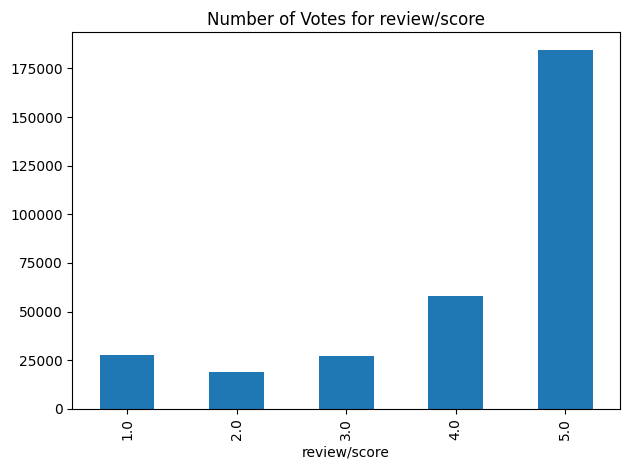
\includegraphics[width=0.4\textwidth]{./figures/h3_votes_distribution.png}
    \caption{Distribution of votes across the four rating categories}
    \label{fig:h3_votes_distribution}
\end{figure}

\noindent
The Spearman correlation coefficient between the two variables is $0.5247$, with a p-value of $0.0$.\\
\textbf{Conclusion:}
The hypothesis is confirmed as there is a positive and statistically significant correlation between the review rating
and helpfulness score. This finding is further supported by the boxplot in Figure \ref{fig:h3_boxplot}.

\begin{figure}[H]
    \centering
    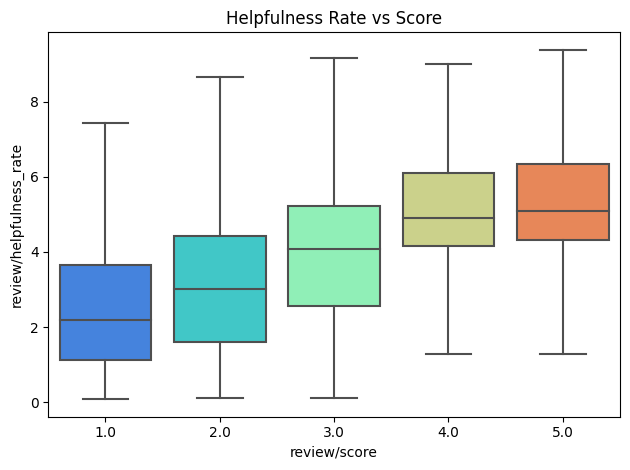
\includegraphics[width=0.3\textwidth]{./figures/h3_boxplot.png}
    \caption{Boxplot illustrating the correlation between review rating and helpfulness score}
    \label{fig:h3_boxplot}
\end{figure}
